\documentclass[border=3pt]{standalone}
\usepackage{tikz}
\usetikzlibrary{shapes, positioning, calc}

\definecolor{fieldfill}{RGB}{222,240,241}
\definecolor{fieldblue}{RGB}{0,0,210}
\definecolor{bitpurple}{RGB}{190,0,70}
\definecolor{logicteal}{RGB}{0,110,110}

\begin{document}
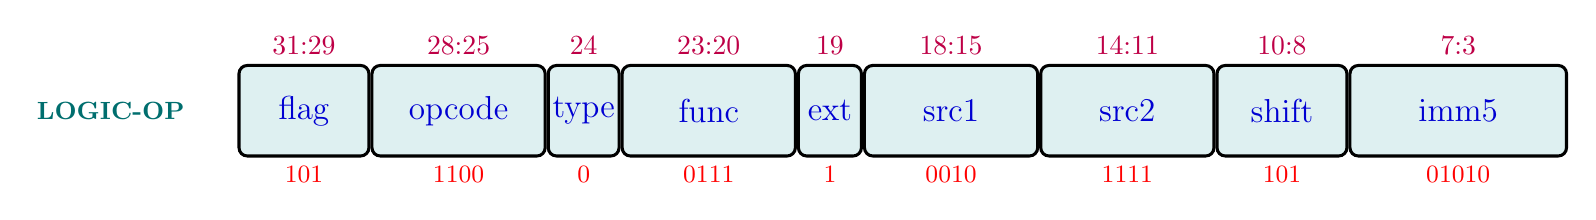
\begin{tikzpicture}[
  field/.style={rectangle, rounded corners=3pt, draw=black, line width=1.1pt, fill=fieldfill, minimum height=1.15cm, inner sep=1pt, align=center, text=fieldblue, font=\large},
  bitlabel/.style={font=\normalsize, text=bitpurple},
  binlabel/.style={font=\small, text=red},
  oplabel/.style={font=\small\bfseries, text=logicteal}
]

% Boxes, sized by bit-field width and touching edge-to-edge
\node[field, minimum width=1.65cm] (flag) {flag};
\node[field, minimum width=2.20cm, anchor=west] (opcode) at (flag.east) {opcode};
\node[field, minimum width=0.90cm, anchor=west] (type) at (opcode.east) {type};
\node[field, minimum width=2.20cm, anchor=west] (func) at (type.east) {func};
\node[field, minimum width=0.80cm, anchor=west] (ext) at (func.east) {ext};
\node[field, minimum width=2.20cm, anchor=west] (src1) at (ext.east) {src1};
\node[field, minimum width=2.20cm, anchor=west] (src2) at (src1.east) {src2};
\node[field, minimum width=1.65cm, anchor=west] (shift) at (src2.east) {shift};
\node[field, minimum width=2.75cm, anchor=west] (imm5) at (shift.east) {imm5};

% Bit-position labels
\node[bitlabel] at ([yshift=0.23cm]flag.north) {31:29};
\node[bitlabel] at ([yshift=0.23cm]opcode.north) {28:25};
\node[bitlabel] at ([yshift=0.23cm]type.north) {24};
\node[bitlabel] at ([yshift=0.23cm]func.north) {23:20};
\node[bitlabel] at ([yshift=0.23cm]ext.north) {19};
\node[bitlabel] at ([yshift=0.23cm]src1.north) {18:15};
\node[bitlabel] at ([yshift=0.23cm]src2.north) {14:11};
\node[bitlabel] at ([yshift=0.23cm]shift.north) {10:8};
\node[bitlabel] at ([yshift=0.23cm]imm5.north) {7:3};

% Binary representation
\node[binlabel] at ([yshift=-0.22cm]flag.south) {101};
\node[binlabel] at ([yshift=-0.22cm]opcode.south) {1100};
\node[binlabel] at ([yshift=-0.22cm]type.south) {0};
\node[binlabel] at ([yshift=-0.22cm]func.south) {0111};
\node[binlabel] at ([yshift=-0.22cm]ext.south) {1};
\node[binlabel] at ([yshift=-0.22cm]src1.south) {0010};
\node[binlabel] at ([yshift=-0.22cm]src2.south) {1111};
\node[binlabel] at ([yshift=-0.22cm]shift.south) {101};
\node[binlabel] at ([yshift=-0.22cm]imm5.south) {01010};

% LOGIC-OP label
\node[oplabel, left=0.55cm of flag] {LOGIC-OP};

\end{tikzpicture}
\end{document}
